\section{\emph{Raspberry PI}}
\label{sec:raspberrypi}
Dieser Abschnitt behandelt den Aufbau von \emph{RPISec} und die verwendete Hardware. Für den Testaufbau wurden folgende Hardwarekomponenten verwendet.
\begin{itemize}
	\item Ein \emph{Raspberry PI 3 Model B}\footnote{\url{https://www.raspberrypi.org/products/raspberry-pi-3-model-b/}},
	\item \emph{AZDeliveryCamRasp}\footnote{\url{https://az-delivery.de/products/raspberrykamerav1-3}} und ein
	\item \emph{HC-SR501\footnote{\url{https://www.mpja.com/download/31227sc.pdf}} Bewegungssensor}.
\end{itemize}
\begin{figure}[h]
	\centering
	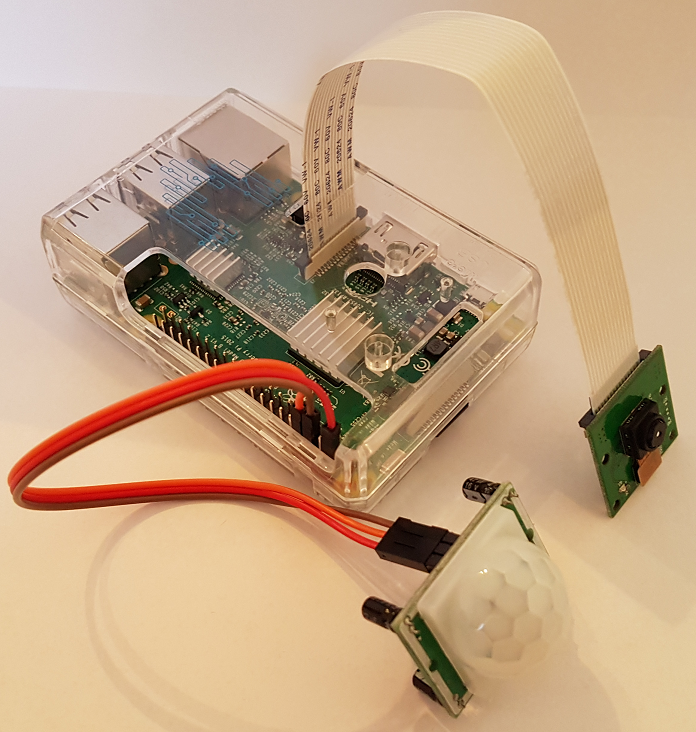
\includegraphics[scale=0.45]{\imageDir/rpisec-hardware-setup.png}
	\caption{Testaufbau der Applikation}
	\label{fig:image-hardware-setup}
\end{figure}
\ \newline
Die Abbildung \ref{fig:image-hardware-setup} zeigt den verwendeten Testaufbau. Die Kamera wurde über CSI \emph{(Camera-Serial-Interface)}) und der Bewegungssensor über GPIO \emph{(General Purpose Input/Output)} an den \emph{Raspberry PI} angeschlossen.

\subsection{Kamera}
Bei der Kamera handelt es sich um ein eigens für den \emph{Raspberry Pi} entwickeltes Modell und wird direkt an den vorhanden Kamera-Port (CSI) des \emph{Raspberry Pi} 3\footnote{\url{https://en.wikipedia.org/wiki/Raspberry_Pi\#/media/File:Raspberry-Pi-3-Flat-Top.jpg}} angeschlossen. Anschließend muss die Kamera aktiviert werden. Dies geschieht über das, mit den meisten Linux-Distributionen mitgelieferte, Programm \emph{raspi-config\footnote{\url{https://upload.wikimedia.org/wikipedia/commons/e/ed/Raspi-config.png}}}. Dieses Programm wird auch benutzt, um andere Komponenten des \emph{Raspberry Pi} zu konfigurieren.
\newpage
\begin{figure}[h]
	\centering
	\includegraphics[scale=0.30]{\imageDir/rpi-border-cam.jpg}
	\caption{Raspberry-Pi 3}
	\label{fig:rpi-border-cam}
\end{figure}
\ \newline
Die Abbildung \ref{fig:raspi-config-cam} zeigt die Oberfläche, über welche die Kamera aktiviert werden kann.
\begin{figure}[h]
	\centering
	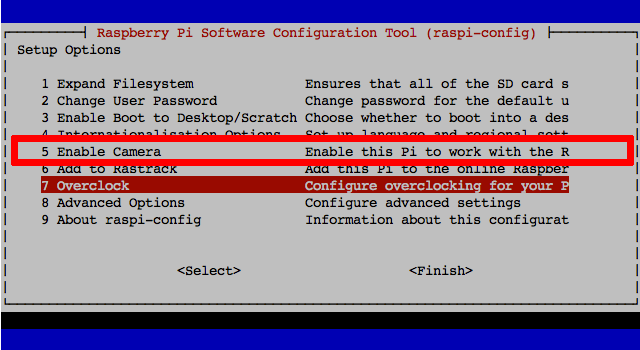
\includegraphics[scale=0.60]{\imageDir/raspi-config-cam.png}
	%By Onepiece84 (Own work) [CC BY-SA 4.0 (http://creativecommons.org/licenses/by-sa/4.0)], via Wikimedia Commons
	\caption{Raspi-config}
	\label{fig:raspi-config-cam}
\end{figure}
\ \newline
Zur Ansteuerung der Kamera wird das Konsolenprogramm \emph{raspistill} verwendet. Diese kann mit verschiedensten Parametern konfiguriert werden. Als Beispiel:
\begin{minted}{bash}
	raspistill --width 1920 --height 1080 -o test.jpg
\end{minted}
Dies erzeugt ein Bild in der Auflösung 1920 x 1080 Pixel und speichert es unter dem Dateinamen \emph{test.jpg}. \emph{RPISec} wird in \emph{Docker Containern} gehostet und die Anwendung \emph{raspistill} wird in ein \emph{Docker Image} installiert und muss daher nicht am Host installiert werden.
\newpage

\subsection{HC-SR501 Bewegungssensor}
Der HC-SR501 Sensor wird über die \emph{GPIO-Pins} des \emph{Raspberry Pi} angesteuert. Hierbei werden Masse, Stromversorgung und Daten-Pin des HC-SR501 Sensors mit den \emph{GPIO-Pins} verbunden. 

\begin{figure}[h]
	\centering
	\includegraphics[scale=0.30]{\imageDir/rpi-border-gpio.jpg}
	\caption{Raspberry-Pi 3}
	\label{fig:rpi-border-gpio}
\end{figure}

Die Pin-Belegung\footnote{\url{http://www.netzmafia.de/skripten/hardware/RasPi/Projekt-PIR/}} des HC-SR501

\begin{figure}[h]
	\centering
	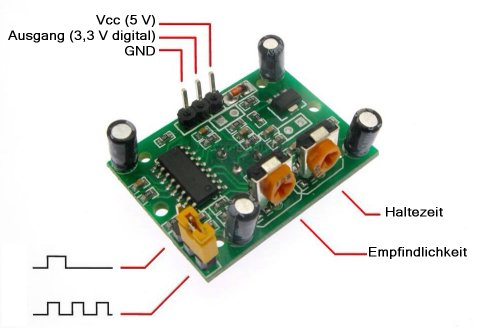
\includegraphics[scale=0.60]{\imageDir/PIR4.jpg}
	\caption{Pin-Schema HC-SR501}
	\label{fig:PIR4}
\end{figure}

ist wie folgt definiert:
\begin{itemize}
	\item Pin 1: VCC (5 Volt)
	\item Pin 2: Out, Data
	\item Pin 3: GND, Masse
\end{itemize}
\ \newpage
Zusätzlich kann die Empfindlichkeit und Haltezeit an den beiden Drehreglern eingestellt werden. Zusätzlich kann noch das Daten-Pin Verhalten über den Jumper konfiguriert werden.

\subsection{GPIO}
\emph{GPIO} ist die Abkürzung für \emph{General Purpose Input/Output}. Man bezeichnet damit programmierbare Ein- und Ausgänge für allgemeine Zwecke. Die \emph{GPIOs} werden als Lötpunkt oder Pin in Form einer Stiftleiste herausgeführt und dienen als Schnittstelle zu anderen Systemen oder Schaltungen, um diese über den \emph{Raspberry Pi} zu steuern. Dabei kann der \emph{Raspberry Pi} bei entsprechender Programmierung digitale Signale von außen annehmen \emph{(Input)} oder Signale nach außen abgeben \emph{(Output)}.
\newline
\newline
Viele der \emph{GPIOs} erfüllen je nach Einstellung und Programmierung verschiedene Funktionen. Neben den typischen \emph{GPIO}-Ein- und Ausgängen finden sich aber auch Pins mit der Doppelfunktion für \emph{I2C, SPI} und eine serielle Schnittstelle.

\subsubsection{HC-SR501 GPIO Verbindung}
Für den HC-SR501 wird die Pin-Belegung wie folgt gewählt:

\begin{itemize}
	\item Pin 1: VCC (5 Volt) an Pin 2
	\item Pin 2: Out, Data an Pin 8
	\item Pin 3: GND an Pin 6
\end{itemize}
\ \newline
Diese Pin-Belegung erfolgt aufgrund der folgenden schematischen Darstellung\footnote{\url{http://pi4j.com/pins/model-3b-rev1.html}}:

\begin{figure}[h]
	\centering
	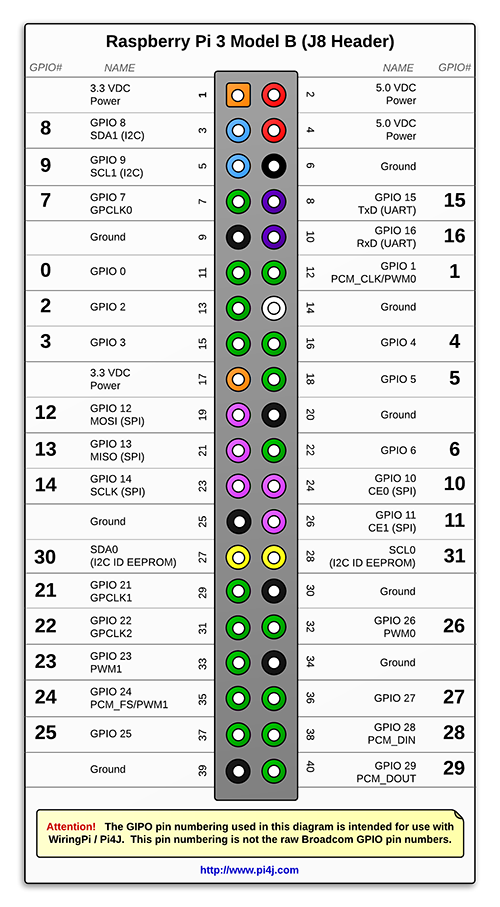
\includegraphics[scale=1.30]{\imageDir/j8header-3b.png}
	\caption{Pin-Schema}
	\label{fig:j8header-3b}
\end{figure}
\newpage

\subsection{Betriebssysteme}
Dieser Abschnitt behandelt die verwendete Betriebssysteme für den \emph{Raspberry PI}. Die Applikation \emph{RPISec} wurde einerseits mit dem Betriebssystem \emph{HypriotOS} und andererseits mit \emph{Raspian} realisiert. Das Betriebssystem \emph{HypriotOS} basiert auf \emph{Debian Jessie} und wird von dem \emph{OpenSource} Projekt \emph{Hypriot}\footnote{\url{https://blog.hypriot.com/}} zur Verfügung gestellt. Das Ziel von \emph{HypriotOS} ist es ein Betriebssystem für den \emph{Raspberry PI} zur Verfügung stellen, das bereits Docker vorinstalliert und betriebsbereit hat. Mit dem Betriebssystem \emph{Raspian} muss Docker selbst installiert werden, wobei Docker als Paket im \emph{Repository} zur Verfügung steht und daher sich die Installation als unkompliziert gestaltet.
\newline
\newline
Wenn Docker installiert und betriebsbereit ist, dann spielt es keine Rolle auf welchem Betriebssystem die Applikation \emph{RPISec} betrieben wird, solange dieses Betriebssystem auf einer von \emph{Docker} unterstützten Kernelversion aufbaut.
\newline
\newline
Da die Applikation \emph{RPISec} auf eine aktive Internetverbindung angewiesen ist, muss das Betriebssystem so konfiguriert werden, dass der \emph{Raspberry PI} entweder über \emph{Ethernet} oder \emph{Wlan} an ein Netzwerk angebunden ist, das Zugriff auf das Internet erlaubt. In einem produktiven Betrieb muss der \emph{Raspberry PI} über das Internet erreichbar sein, damit die mobilen \emph{Clients} Anfragen an die gehosteten \emph{Microservice} absetzen können.
\begin{figure}[h]
	\centering
	
\includegraphics[scale=0.5]{\imageDir/hypriot-logo.jpg}
	\caption{HypriotOS}
	\label{fig:HypriotOS}
\end{figure}\begin{figure}[h]
	\centering
	
\includegraphics[scale=0.15]{\imageDir/raspbian-logo.png}
	\caption{RaspianOS}
	\label{fig:RaspianOS}
\end{figure}